%%%%%%%%%%%%%%%%%%%%%%%%%%%%%%%%%%%%%%%%%%%%%%
% An example of a lab report write-up.
%%%%%%%%%%%%%%%%%%%%%%%%%%%%%%%%%%%%%%%%%%%%%% 
% This is a combination of several labs that I have done in the past for 
% Computer Engineering, so it is not to be taken literally, but instead used as 
% a great starting template for your own lab write up.  When creating this 
% template, I tried to keep in mind all of the functions and functionality of 
% LaTeX that I spent a lot of time researching and using in my lab reports and 
% include them here so that it is fairly easy for students first learning LaTeX
% to jump on in and get immediate results.  However, I do assume that the 
% person using this guide has already created at least a "Hello World" PDF 
% document using LaTeX (which means it's installed and ready to go). 
%
% My preference for developing in LaTeX is to use the LaTeX Plugin for gedit in 
% Linux.  There are others for Mac and Windows as well (particularly MikTeX).  
% Another excellent plugin is the Calc2LaTeX plugin for the OpenOffice suite.  
% It makes it very easy to create a large table very quickly.  
%
% Professors have different tastes for how they want the lab write-ups done, so 
% check with the section layout for your class and create a template file for 
% each class (my recommendation).
%
% Also, there is a list of common commands at the bottom of this document.  Use
% these as a quick reference.  If you'd like more, you can view the "LaTeX Cheat
% Sheet.pdf" included with this template material. 
%
% (c) 2009 Derek R. Hildreth <derek@derekhildreth.com> http://www.derekhildreth.com 
% This work is licensed under the Creative Commons Attribution-NonCommercial-ShareAlike License. To view a copy of this license, visit http://creativecommons.org/licenses/by-nc-sa/1.0/ or send a letter to Creative Commons, 559 Nathan Abbott Way, Stanford, California 94305, USA.
%%%%%%%%%%%%%%%%%%%%%%%%%%%%%%%%%%%%%%%%%%%%%%

\input kvmacros % For Karnaugh Maps (K-Maps)
\documentclass[UTF8]{ctexart}
\usepackage{graphicx} % For images
\usepackage{float}    % For tables and other floats
\usepackage{verbatim} % For comments and other
\usepackage{amsmath}  % For math
\usepackage{amssymb}  % For more math
\usepackage{fullpage} % Set margins and place page numbers at bottom center
\usepackage{listings} % For source code
\usepackage{subfig}   % For subfigures
\usepackage[usenames,dvipsnames]{color} % For colors and names
\usepackage{hyperref}           % For hyperlinks and indexing the PDF
\hypersetup{ % play with the different link colors here
    colorlinks,
    citecolor=blue,
    filecolor=blue,
    linkcolor=blue,
    urlcolor=blue % set to black to prevent printing blue links
}

\definecolor{mygrey}{gray}{.96} % Light Grey
\lstset{ 
	language=[ISO]C++,              % choose the language of the code ("language=Verilog" is popular as well)
   tabsize=3,							  % sets the size of the tabs in spaces (1 Tab is replaced with 3 spaces)
	basicstyle=\tiny,               % the size of the fonts that are used for the code
	numbers=left,                   % where to put the line-numbers
	numberstyle=\tiny,              % the size of the fonts that are used for the line-numbers
	stepnumber=2,                   % the step between two line-numbers. If it's 1 each line will be numbered
	numbersep=5pt,                  % how far the line-numbers are from the code
	backgroundcolor=\color{mygrey}, % choose the background color. You must add \usepackage{color}
	%showspaces=false,              % show spaces adding particular underscores
	%showstringspaces=false,        % underline spaces within strings
	%showtabs=false,                % show tabs within strings adding particular underscores
	frame=single,	                 % adds a frame around the code
	tabsize=3,	                    % sets default tabsize to 2 spaces
	captionpos=b,                   % sets the caption-position to bottom
	breaklines=true,                % sets automatic line breaking
	breakatwhitespace=false,        % sets if automatic breaks should only happen at whitespace
	%escapeinside={\%*}{*)},        % if you want to add a comment within your code
	commentstyle=\color{BrickRed}   % sets the comment style
}

% Make units a little nicer looking and faster to type
\newcommand{\Hz}{\textsl{Hz}}
\newcommand{\KHz}{\textsl{KHz}}
\newcommand{\MHz}{\textsl{MHz}}
\newcommand{\GHz}{\textsl{GHz}}
\newcommand{\ns}{\textsl{ns}}
\newcommand{\ms}{\textsl{ms}}
\newcommand{\s}{\textsl{s}}



% TITLE PAGE CONTENT %%%%%%%%%%%%%%%%%%%%%%%%
% Remember to fill this section out for each
% lab write-up.
%%%%%%%%%%%%%%%%%%%%%%%%%%%%%%%%%%%%%%%%%%%%%

\newcommand{\labtitle}{PCA KPCA LLE}
\newcommand{\authorname}{李梓铉}
\newcommand{\professor}{孟德宇教授}
\newcommand{\classno}{3118103163}
% END TITLE PAGE CONTENT %%%%%%%%%%%%%%%%%%%%


\begin{document}  % START THE DOCUMENT!


% TITLE PAGE %%%%%%%%%%%%%%%%%%%%%%%%%%%%%%%%%%%%%%
% If you'd like to change the content of this,
% do it in the "TITLE PAGE CONTENT" directly above
% this message
%%%%%%%%%%%%%%%%%%%%%%%%%%%%%%%%%%%%%%%%%%%%%%%%%%%
\begin{titlepage}
\begin{center}
{\LARGE \textsc{机器学习降维方法实验报告 :} \\ \vspace{4pt}}
{\Large \textsc{\labtitle} \\ \vspace{4pt}} 
\rule[13pt]{\textwidth}{1pt} \\ \vspace{150pt}
{\large  \authorname \\ \vspace{10pt}
学号 \classno\\ \vspace{10pt}
指导老师: \professor \\ \vspace{10pt}
\today}
\end{center}
\end{titlepage}
% END TITLE PAGE %%%%%%%%%%%%%%%%%%%%%%%%%%%%%%%%%%





%%%%%%%%%%%%%%%%%%%%%%%%%%%%%%
%%%%%%%%%%%%%%%%%%%%%%%%%%%%%%
\section{实验背景}
%No Text Here
%%%%%%%%%%%%%%%%%%%%%%%%%%%%%%%
\subsection{实验目的}
\begin{comment}
This is a lab template which has a ton of different things which are useful in writing lab write-ups in the Computer Eningeering field.  This is demonstrating the comment block. Don't be overwhelmed, it may seem like a lot to take in at a time, but it's worth spending the time learning it.
\end{comment}
机器学习通常需要大量的训练样本,而在现实中得到的数据通常很难满足训练样本的密集采样,而且属性维度的增加若满足采样条件,会使得样本的数字达到天文数字。在高维情形下出现的数据样本稀疏,巨大的矩阵导致的计算距离困难等等,就是机器学习方法面临的严重障碍“维数灾难”(curse of dimensionality). 解决维数灾难的重要方法之一是降维(dimension reduction),通过数学变换将高维空间转变为一个低维子空间使得样本密度提高,降低距离计算的复杂度。一般来说有效的降维方法要保持前后的样本之间的距离。\vspace{3mm} 

降维的方法主要分为两类:\vspace{3mm} 

第一类也是降维最简单的方法就是基于线性变换的线性降维方法,多维缩放(MDS),主成分分析(PCA) 算法均属于此类降维方法。线性降维方法是高维到低维空间的线性映射,但对于现实任务中的很多数据,需要使用非线性映射才能找到适当的低维嵌入。\vspace{3mm} 

第二类方法就是非线性方法,非线性方法中的第一种是核化线性降维,如核主成分分析(KPCA),使用核函数,将高维特征空间中得数据投影到一个超平面上实现降维。第二种是流形学习(manifold learning),这是一种借鉴拓扑流形概念的降维方法。低维流形嵌入到高维空间的分布虽然很复杂,但局部仍然具有欧式空间的性质,因此可以在局部建议降维映射关系,然后在推广至全局。著名的流形学习方法有等度量映射(Isometric mapping)Isomapping,局部性嵌入(local linear embedding)LLE等。\vspace{3mm} 


在本文中,将使用PCA,Kpca,Isomap,LLE四种方法对随机生成的高维数据进行降维。通过实验了解各类降维方法的特点,在理解原理的基础上对各类方法有更直观的认识,然后再对一个现实工程问题进行方法的应用。报告将包含以下5个主要部分:
\begin{itemize}
	\item 主成分分析方法(PCA)
	\item 核主成分分析方法(KPCA) 
	\item 局部性嵌入(LLE)
	\item 工程应用
	\item 结论与讨论
\end{itemize}
\vspace{3mm}  

%%%%%%%%%%%%%%%%%%%%%%%%%%%%%%
\subsection{编译环境}
使用python语言进行实验,相关的编译环境如下:
	\begin{itemize}
		\item 操作系统Windows 10
		\item python3.6编译器
		\item scikit-learn 0.20.1 (机器学习python库)
		\item numpy (python数组处理库)
		\item matplotlib(python可视化库)
	\end{itemize}

%%%%%%%%%%%%%%%%%%%%%%%%%%%%%%
%\subsection{Procedure}

%	\begin{enumerate}
%		\item Start the ISE Navigator. See the ISE 8.2i Quick Start Tutorial.
%		\item Create a new project.
%		\item Import copies of the Verilog modules AND\_OR, MY\_AND2, and MY\_OR2 to the new project just created.
%		\item Create a Test Bench (called Test Fixture in Verilog).
%		\item Create the actual input stimulus.
%		\item Run the simulation, examine the waveforms, and verify functioniality.
%	\end{enumerate}

%%%%%%%%%%%%%%%%%%%%%%%%%%%%%%
%%%%%%%%%%%%%%%%%%%%%%%%%%%%%%
\newpage
\section{PCA}
\subsection{方法介绍}
主成分分析(Principal Component Analysis)是最常用的一种降维方法。PCA通过用一个超平面对正交空间中的所有样本点进行近似表达。这个超平面要满足两点:1. 重构性:样本点到这个超平面的距离都足够近。 2.最大可分性:样本点在这个超平面上的投影能尽可能分开。\vspace{3mm}  


算法的主要过程可以总结如下:



\begin{enumerate}
	\item 输入:样本集D,期望的低维空间维数n。
	\item 对所有样本进行中心化。
	\item 计算样本的协方差矩阵。
	\item 对协方差矩阵做特征值分解。
	\item 排序特征值取最大的n个特征值所对应的特征向量。
	\item 输出:特征向量对应的投影矩阵
\end{enumerate}



降维后的低维空间的维数由使用者决定,可以通过选不同的维数通过交叉验证得到较好的维数n,显然在PCA过程中,较小的特征值对应的特征向量对应的信息被舍弃了,这是降维的必要结果,因为较小的特征值对应的信息往往是无用的噪声信息,舍弃后可以使样本采样密度增大,一定程度上起到去噪的效果。

\subsection{实验介绍}
仿照sci-kit示例程序,本实验使用numpy生成三个随机数组,将数组通过线性变化,变换为三维空间中的点云,点云分布有显著的接近一个平面(x-y-z=0)上分布的特征。然后程序通过调用sci-kit的PCA程序,设置低维空间维数为3,得到一个超平面(近似平面x-y-z=0)来近似所有的样本点,并进行了可视化。

可视化结果如下。

	\begin{figure}[H]
	  \centering
	  \label{fig:Per6A}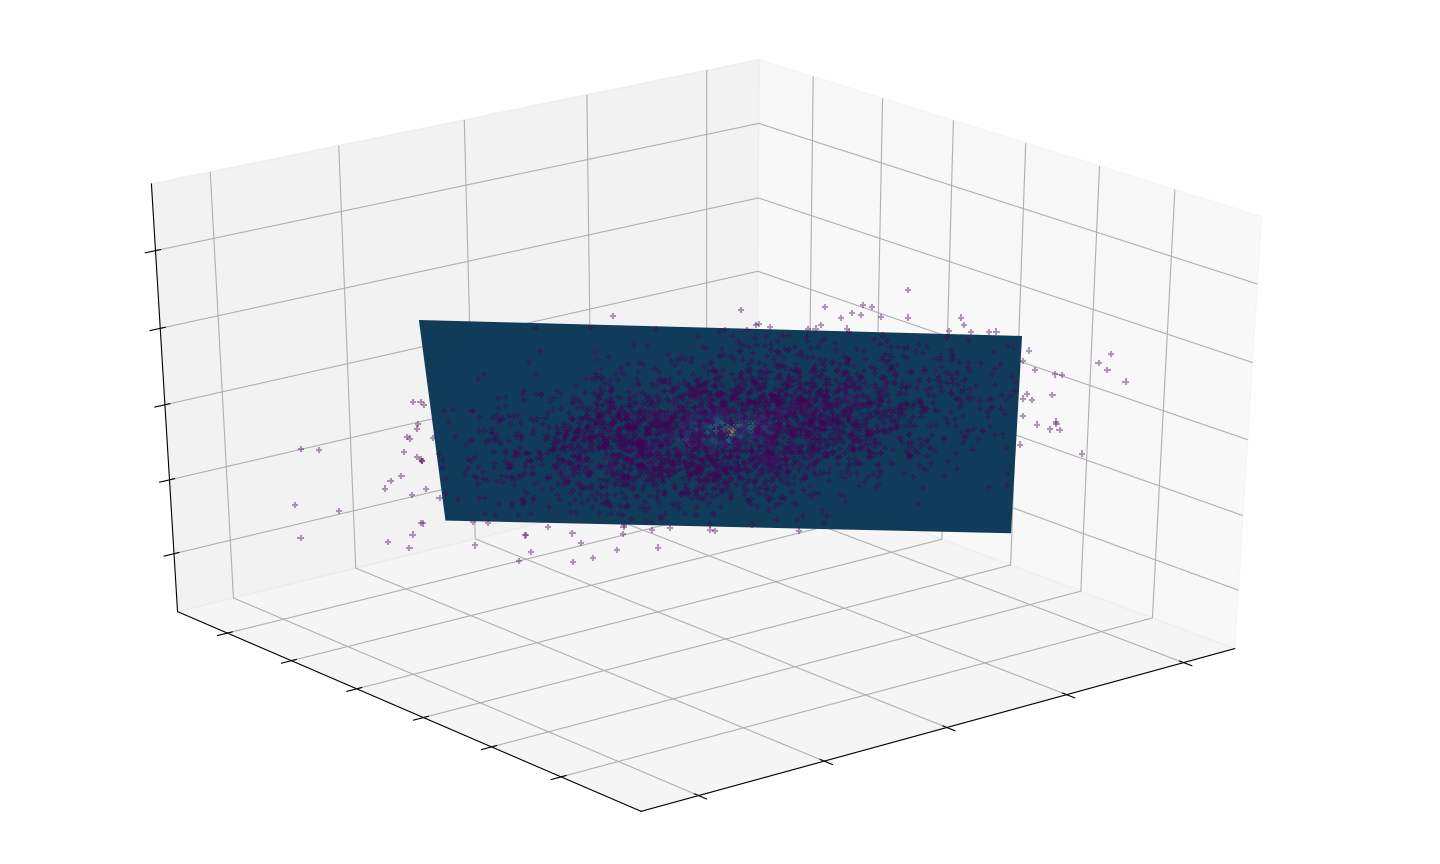
\includegraphics[width=0.4\textwidth]{pca.png}\
	  \caption{PCA点云近似可视化结果}
	  \label{fig:oscil}    
	\end{figure}

\subsection{源代码}
实验使用的源代码如下.  \vspace{5mm}
	\lstinputlisting{plot_pca_3d.py}
	\vspace{3mm}






\newpage
\section{KPCA}
\subsection{方法介绍}
核主成分分析(Principal Component Analysis)是核化线性降维的一种方法。核函数是一种数学技巧变换技巧,可以将样本映射到一个高维特征空间去。KPCA使用核函数可以对样本进行非线性的映射再做降维处理。KPCA的优势在于,映射后的数据集在映射后通常可以保留聚类特征,有时对于扭曲的流形数据集也有很好的效果。KPCA常用的核函数有Gaussian Radial Basis Function (RBF)核函数。Gaussian RBF Function如下:

\begin{align*}
		\phi \gamma(x,\iota) = exp(-\gamma \lVert x-l \rVert ^2)\\
\end{align*}

通过将数据集的每一个样本用核函数映射到一个高维特征空间去。相比原来的样本,新样本会有很多新的维度,同时也因此提高了数据集线性可分的概率。然后再在特征空间中实施PCA即可。核化的弊端在于训练集如果很大的话,那么核化后的数据的feature将非常多,并且为了获得投影,KPCA要对所有样本求和,计算开销较大。
\vspace{3mm}  

算法的主要过程可以总结如下:



\begin{enumerate}
	\item 输入:样本集D,期望的低维空间维数n,核函数$\phi$
	\item 得到样本在高维特征空间的像。
	\item 实施PCA
	\item 输出:特征向量对应的投影矩阵
\end{enumerate}




\subsection{实验介绍}
仿照sci-kit示例程序,本实验使用scikit的datasets库方法,生成两组sample,在x1,x2空间上分布近似为两个同心圆。先调用了PCA,对样本进行了处理并输出了最大特征值对应的两个特征向量下的样本空间。然后调用scikit的K\_pca方法,使用rbf\_kernel,对样本进行了处理。并输出了最大的两个特征值对应的特征向量描述的样本空间。然后输出了在原x1,x2空间中,经过KPCA处理的样本。
可视化结果如下。

	\begin{figure}[H]
	  \centering
	  \label{fig:Per3A}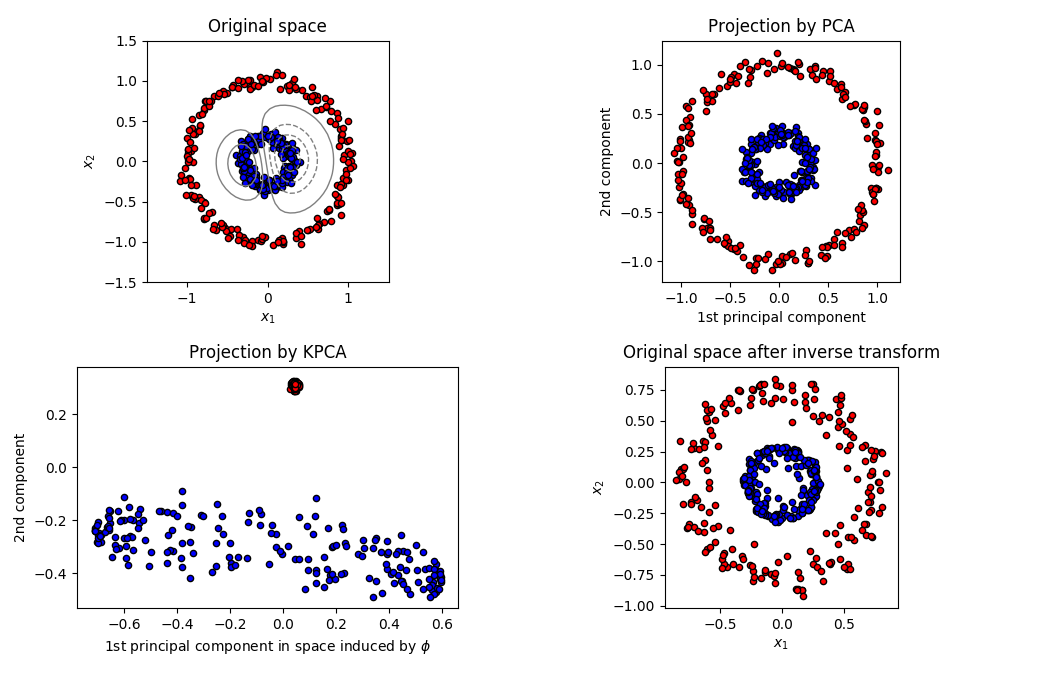
\includegraphics[width=0.8\textwidth]{Kpca.png}\
	  \caption{KPCA可视化结果}
	  \label{fig:oscil}    
	\end{figure}
	
可以看出从图Projection by KPCA看出,经过KPCA处理,新的样本变的线性可分了,并且根据Original space after inverse transform可以看出,KPCA很好的保留了样本的原始聚类特征。而从Projection by PCA可以看出,线性降维后的样本和原来的样本很接近,并没有提取出样本中的聚类特征。

\subsection{源代码}
实验使用的源代码如下.  \vspace{5mm}
	\lstinputlisting{plot_kernel_pca.py}
	\vspace{3mm}




\newpage
\section{LLE}
\subsection{方法介绍}
局部线性嵌入(Locally Linear Embedding, 简称LLE)是流形学习的一种。与Isomap通过建立临近连接图再使用MDS方法降维的方法不同,LLE方法通过保持邻域样本之间的线性关系降维。即一个样本$x_1$可以通过邻域样本$x_i,x_j,x_k$线性表示的话,那么经过LLE降维后,该关系将继续保持。这使得LLE算法对于卷曲的manifold数据的处理非常有效,尤其是当噪声较小的时候。\vspace{3mm}  

算法的主要过程可以总结如下:


\begin{enumerate}
	\item 输入:样本集$D={x_1,x_2,...,x_m}$,期望的低维空间维数n,临近参数k
	\item for i = 1,2,...,m do
	\item 确定$x_i$的k临近
	\item 通过$\min\limits_{1,...,m} \sum_{i = 1} ^m(\lVert x_i - \sum\limits_{j \in Q_i }(w_{ij}  x_j) \rVert)^2$ 求得对$x_i$线性重构的系数$w_ij$,$j \in Q_i$
	\item 对于$j \notin Q_i$,令$w_{ij}=0$
	\item endfor
	\item $M=(I-W)^T(I-W)$
	\item 对M进行特征分解
	\item 返回M的最小的n个特征值的特征向量
	\item 输出:样本集在特征向量对应的低维空间的投影
\end{enumerate}


但由于LLE算法先要寻找k邻近$O(mlog(m)nlog(k))$,再计算wight矩阵$O(mnk^3)$,然后建立低维度的表示$O(m^2)$。最后一项的计算复杂度$(m^2)$导致LLE对于大型的数据集的计算基本是无能为力的。
\subsection{实验介绍}
仿照sci-kit示例程序,本实验使用scikit的datasets库方法,生成经典的manifolding 数据“瑞士卷”样本,在空间中呈现卷曲的状态。然后使用LLE方法对数据样本进行了处理,输出了在新的低维空间上的数据分布。可视化结果如下:

	\begin{figure}[H]
	  \centering
	  \label{fig:Per3A}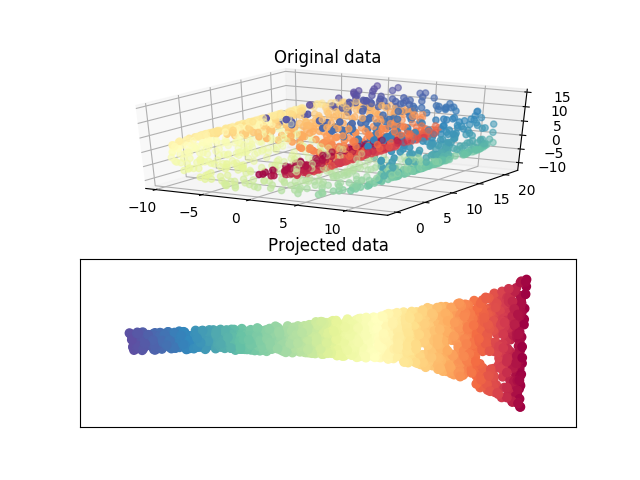
\includegraphics[width=0.8\textwidth]{LLE.png}\
	  \caption{LLE可视化结果}
	  \label{fig:oscil}    
	\end{figure}
	
可以看出从图中看出,LLE方法很好的实现了对manifolding数据在低维空间的展开。

\subsection{源代码}
实验使用的源代码如下.  \vspace{5mm}
	\lstinputlisting{plot_swissroll.py}
	\vspace{3mm}




\newpage
\section{工程应用}
\subsection{背景介绍}
前文的样本均为人为产生的,有很好的特征可供演示各类算法的特点。本节将对实际工程中得信号进行降维,以达到工程目的。\\
旋转机械属于能源与动力工程领域中使用较为广泛的机械设备,而转子是其核心部件。转子系统在运行过程中的振动信号会因裂纹故障发生显著的的变化。本节通过使用机器学习方法,对Case Western Reserve University Bearing Data Center Website上的转子故障数据,实现对转子故障的分析诊断。
实验使用一台2hp Reliance电动马达进行,加速度数据在靠近和远离马达轴承的位置进行测量。使用电火花加工( EDM )在电机轴承上播种故障。本研究使用直径为0.007英寸到0.04英寸直径裂纹故障的转子数据。转子数据中包括出现故障的轴承以及正常的轴承安装到测试电机中,电机负载为0至3马力(电机转速为1797至1720 RPM )时的振动数据。共9个类别对应如下。
{'Normal': 0, 'B007': 1,'B014': 2,'B021': 3,'IR007': 4,'IR014': 5,'IR021': 6,'OR007@6': 7,'OR014@6': 8,'OR021@6': 9, }
  数字代表裂纹直径,如007为0.007英寸,字母B,IR(inner race),OR(outer race)代表同一故障实验不同测点处的数据。

	\begin{figure}[H]
	  \centering
	  \label{fig:Per3A}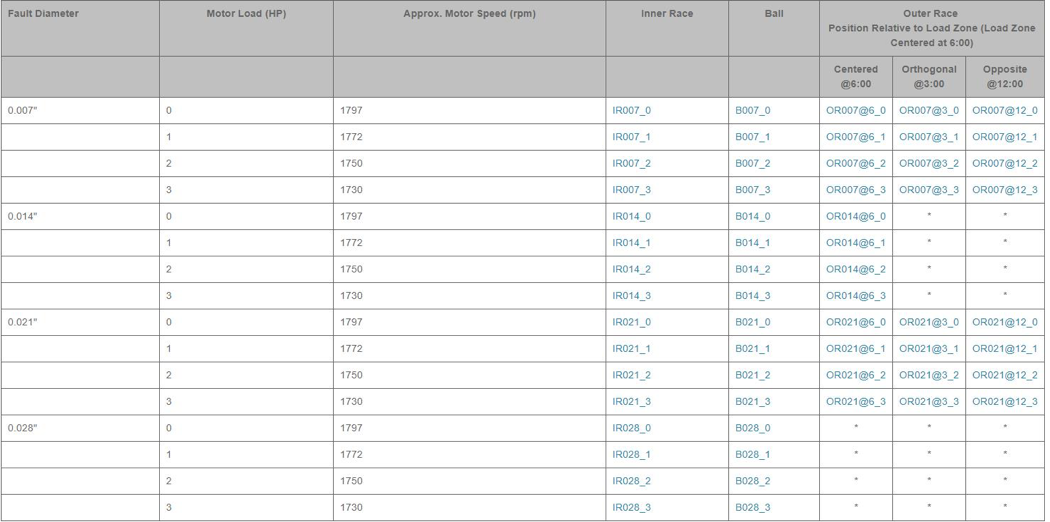
\includegraphics[width=1.0\textwidth]{summary.png}\
	  \caption{故障信息表格}
	  \label{fig:oscil}    
	\end{figure}


\vspace{3mm}  

本研究以0,1,2马力负载时的时序信号作为训练集,3马力负载时的时序信号作为测试集,通过使用PCA降维,然后使用的机器学习算法Logistics Regression,实现multi-label classification任务,并对比降维前后的分类效果。

\subsection{实验介绍}
先对数据进行预处理,过程如下:
\begin{enumerate}
	\item 读入数据(load\_data)
	\item 切割数据(wave\_cut) 通过给定的时间窗大小(2048)和期望的sample数量(256),将一个时序信号切割成对应的sample signal。
	\item 对信号增加白噪声(add\_noise),实现数据增强,使得切割得到的数据更贴近于实际信号。
	\item 归一化(trans\_norm)
	\item FFT快速傅立叶变换(trans\_fft)实际是对数据的一次降维,将时序信号转化为有限个频域上的幅值。
\end{enumerate}
处理后的信号如下图
	\begin{figure}[H]
	  \centering
	  \label{fig:Per3A}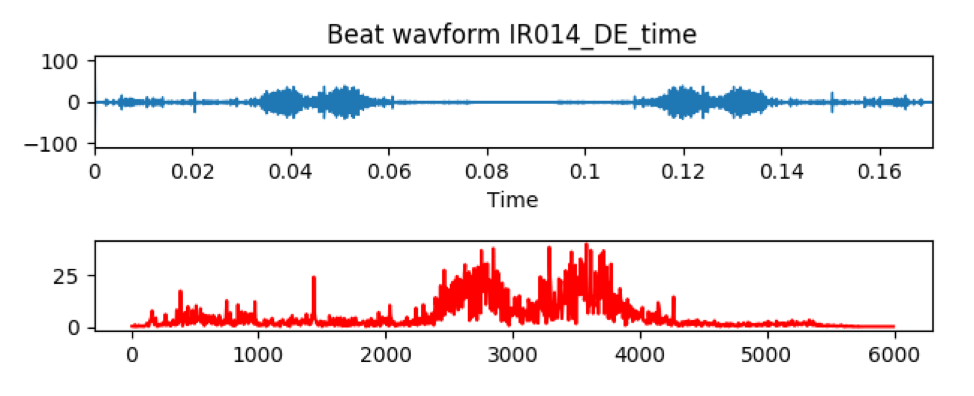
\includegraphics[width=0.8\textwidth]{timesig.png}\
	  \caption{R014\_DE 的时序信号以及频域信号}
	  \label{fig:oscil}    
	\end{figure}
	
	\begin{figure}[H]
	  \centering
	  \label{fig:Per3A}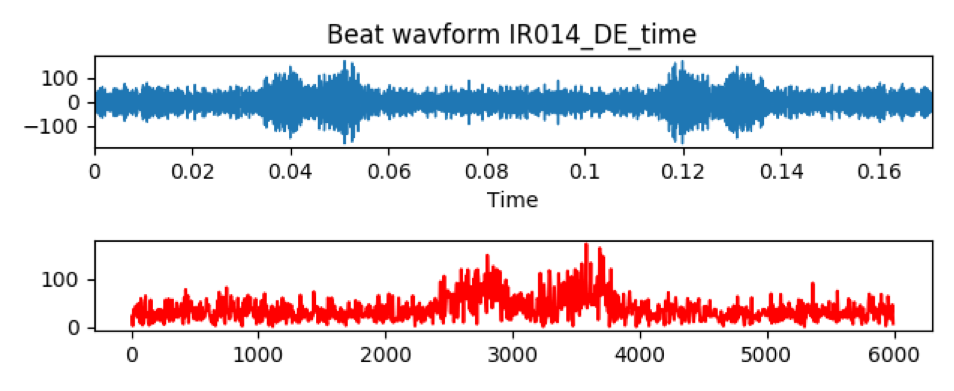
\includegraphics[width=0.8\textwidth]{whitnoise.png}\
	  \caption{R014\_DE 的时序信号以及频域信号}
	  \label{fig:oscil}    
	\end{figure}
	
因为窗函数大小为2048,所以经过傅里叶变换,信号频域大小为1024。但是这些频率显然并不都是与故障相关的,直观上样本间方差较大的频率更有可能包含故障信息,因此对频域信号做PCA (主成分分析)来进一步降维,通过多次试验,取低维空间维数100,将振动数据转化为更低维子空间中信息更密集的样本点。然后分别使用sci\-kit库中的Logistics Regression进行训练和分类。 然后再使用未做PCA的样本进行训练和分类,得到实验结果。

PCA前分类正确率为:0.8826

PCA后分类正确率为:0.9004

可以看出,大幅压缩样本维度后,分类正确率并没有受到影响且有略微的提升。虽然分类正确率没有很高,但达到了基本的分类目的,用于工程实践还需要进一步的优化。


\subsection{源代码}
实验使用的源代码如下。( 省略了data\_read读入数据部分) \vspace{5mm}
	\lstinputlisting{classify.py}
	\vspace{3mm}
	

\newpage
\section{结论与讨论}
实验的目的是通过使用代码,了解如何使用降维方法对数据进行降维,熟悉相关的编程环境以及调用方式。底层的算法实现并不是本实验的要求。

本文通过使用Sci-kit learn python库实现了三种机器学习算法的实验,尽管没有从最底层的代码进行实现,但是经过实验实现了三种降维算法的应用。PCA属于线性降维方法,KPCA属于非线性降维方法,LLE属于非线性降维方法中的流形学习方法。并对一个工程实际数据进行了分析,实现了基本的分类目标。通过实际的实验,对于降维的意义通过可视化有了更加直观的认识。对于算法原理也有了更深刻的认识。降维的线性与非线性方法的区别与特点也在实验中有所体现。如果之后有时间,会花更多时间,从底层代码完成三种机器学习算法,而不是单纯调库。

报告写作过程中参考了周志华《机器学习》,以及《Hands on machine learning with sci-kit learn》。代码demo部分来源于scikit-learn网站。

最后感谢孟教授这学期的教学,您的课干货满满,深入浅出。只是有些可惜课时太少,很希望未来机器学习这门课可以调整成全周的课程。顺颂时祺。

\end{document} % DONE WITH DOCUMENT!





%%%%%%%%%%%%%%%%%%%%%%%%%%%%%%
\newpage
\section{Experiment Data}
This section will consist of the important code blocks which were changed in order to meet the requirements of the lab.  \vspace{5mm}
	\lstinputlisting{code.c}
	\vspace{3mm}



% IF YOU'D RATHER TYPE THE CODE, OR HAVE A SMALLER BLOCK OF CODE, USE THIS:
%\begin{lstlisting}
%if(something)
%	do this
%else
%	do this
%\end{lstlisting}

%% THIS IS FROM A DIFFERENT CLASS, BUT DEMONSTRATES MATH MODE WELL
%%%%%%%%%%%%%%%%%%%%%%%%%%%%%%
\subsection{Formulas and Overall Descriptions Used}
This part of the laboratory was done for \href{http://www.byui.edu/catalog/2004-2005/class.asp1075.htm}{Feedback Control}.  Most of this laboratory's calculations were completed and compiled by the folks at Quanser (the manufacturer of the inverted pendulum) and will give the lab a good starting place.  Below are the state equation and gain values used initially in the lab:
	\[
	\begin{bmatrix}
	\dot{\alpha} \\
	\ddot{\alpha} \\
	\dot{\theta} \\
	\ddot{\theta} \\
	\end{bmatrix}
	=
	\begin{bmatrix}
	0 & 1 & 0 & 0 \\
	81.7 & 0 & 0 & -13.9 \\
	0 & 0 & 0 & 1 \\
	39.7 & 0 & 0 & -14.4 \\
	\end{bmatrix}
	\begin{bmatrix}
	\alpha \\
	\dot{\alpha} \\
	\theta \\
	\dot{\theta} \\
	\end{bmatrix}
	+
	\begin{bmatrix}
	0 \\ 
	24.5 \\
	0 \\ 
	25.4 \\
	\end{bmatrix}
	V
	\]

	\[
	K  = 
	\begin{bmatrix}
	21 & 2.8 & -2.2 & -2.0 \\
	\end{bmatrix}
	\]

Other values, such as the $\frac{\mbox{Volts}}{\mbox{Degree}}$ and $\frac{\mbox{Degrees}}{\mbox{Volt}}$ were obtained by first determining the max angle of the pendulum on both extreme sides.

Using the max angles from above, these values were determined:
	\[
	\begin{array}{l l}
		\alpha = 0.062 \frac{\mbox{Volts}}{\mbox{Degree}} \\ \\
		\alpha = 15.105 \frac{\mbox{Degrees}}{\mbox{Volt}} \\
	\end{array}
	\]

I would also like to add that in order to calibrate $\alpha$ to get a perfect vertical $= 0$, a value of $0.09$ needed to be added.  The same applies to $\theta$ where $0.322$ needs to be added.

%%%%%%%%%%%%%%%%%%%%%%%%%%%%%%
\subsection{DC Motor Transfer Function and Parameters}

Definitions:
	\begin{align*}
		\theta(t) =  Angular Position \\
		\dot{\theta}(t) =  Angular Velocity \\
		\triangle t = t_{10\%} - t_{90\%} \\
		90\% = e^{-t_{10\%}/\tau} \\
		10\% = e^{-t_{90\%}/\tau} \\ 
	\end{align*}

The Math:
	\begin{align*}
		\frac{s\theta(s)}{V_{a}(s)} = \frac{K}{s+P} \\
		\mbox{Let}\ V_{a}(s) = \frac{V_{0}}{s} \\  % If you'd like to have a space following any command, add "\" to the end as shown here.
		s\theta(s) = \frac{KV_{0}}{(S+P)S} = \frac{KV_{0}}{\frac{P}{S}} - \frac{\frac{KV_{0}}{P}}{s+P} \\
		L^{-1} \Rightarrow \dot{\theta}(t) = \frac{KV_{0}}{P}(1-e^{-t/(1/P)}) \\
		\dot{\theta}(t) = (\dot{\theta}_{i} - \dot{\theta}_{f})e^{-pt} + \dot{\theta}_{f} \\
	\end{align*}

Final equations:
	\begin{align}
		\label{thetadot}\dot{\theta}_{f} = \frac{KV_{0}}{P} \\
		\label{equ:tau}\frac{1}{P} = \tau = \frac{\triangle t}{ln(9)}
	\end{align}

Graphically (Refer to Equation \ref{thetadot} and Equation \ref{equ:tau}) :
	% Drawn and exported to png using Inkscape.
	\begin{figure}[h]
		\begin{center}
			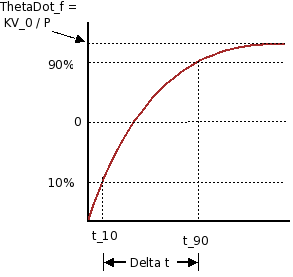
\includegraphics[width=0.33\textwidth]{graph.png}
		\end{center}
	\label{graph}
	\end{figure}

% AGAIN, ANOTHER EXAMPLE FROM A DIFFERENT CLASS WHICH DEMONSTRasdATES KMAPS AND TABLES NICELY.
\newpage % I added this after viewing the completed pdf and decided to make this cosmetic change
This section consists of tables and reductions which were used in this laboratory exercise.

% This table was generated using the Calc2LaTeX macro which I mentioned earlier.
% You'll need OpenOffice installed and you'll have to download the macro online.
% If you're interested, I have a guide on how to set this up and use it on my
% blog.  http://www.derekhildreth.com/blog  Search for "LaTeX".  You'll find it.
	\begin{table}[htbp]
	\begin{center}
		\begin{tabular}{|ccc|cc|}
			\hline
			\textbf{PS} & \textbf{D} & \textbf{N} & \textbf{NS} & \textbf{P} \\ \hline
			\$0.00 & 0 & 0 & \$0.00 & 0 \\
			 & 0 & 1 & \$0.05 & 0 \\ 
			 & 1 & 0 & \$0.10 & 0 \\
			 & 1 & 1 & -- & -- \\ \hline
			\$0.05 & 0 & 0 & \$0.05 & 0 \\ 
			 & 0 & 1 & \$0.10 & 0 \\ 
			 & 1 & 0 & \$0.15 & 0 \\ 
			 & 1 & 1 & -- & -- \\ \hline
			\$0.10 & 0 & 0 & \$0.10 & 0 \\ 
			 & 0 & 1 & \$0.15 & 0 \\ 
			 & 1 & 0 & \$0.15 & 0 \\ 
			 & 1 & 1 & -- & -- \\ \hline
			\$0.15 & -- & -- & \$0.15 & 1 \\ \hline
			\end{tabular}
	\end{center}
	\caption{Symbolic Transition Table}
	\label{symbolic}
	\end{table}

	\begin{table}[H]
		\centering
		\subfloat[D1 = $Q_{1}$+D+$Q_{0}$N] % Caption
			{
				\karnaughmap{4}{D1:}{ {$Q_{1}$} {$Q_{0}$} {D} {N} }{001X011X111X111X}{}  % See the included kvdoc.pdf file for more details 
			} \hspace{10mm} % seperate them a bit
		\subfloat[D0 = $\Bar{Q_{0}}$N + $Q_{0}\Bar{N}$ + $Q_{1}$N + $Q_{1}$D] % Caption
			{
				\karnaughmap{4}{D0:}{ {$Q_{1}$} {$Q_{0}$} {D} {N} }{010X101X011X111X}{}
			}
	  \caption{Karnaugh maps and the simplified results of the logic.}
	  \label{fig:kmaps}
	\end{table}


%%%%%%%%%%%%%%%%%%%%%%%%%%%%%%
%%%%%%%%%%%%%%%%%%%%%%%%%%%%%%
\newpage
\section{Discussion \& Conclusion}
The goal of this lab was to re-design the LED/Switch system to include a hardware timer.  By pressing eight different combinations of the three buttons, the LEDs on the board were to act in different ways using these timers. There was not a Q\&A requirement for this lab. \vspace{3mm} % I use this to seperate the paragraphs a bit.

I was able to accomplish the requirements of the lab by utilizing the \texttt{IntMgrTimerExample.c} project found within the analog devices example programs folder (and mentioned in the class lecture).  There were some stumbling blocks to overcome.  The most difficult for myself was actually getting the period of the LEDs just right.  I was able to get it very close to the 333.3\ms, 666.7\ms, and 1\s periods, but not exactly.  My first method of getting these periods right was to take the clock speed in \MHz, find the period by taking the inverse of the clock speed, and then solving for the value in hex that was needed to get the right period.  This didn't yeild very accurate results at all, and so I then went through a trial and error session until I got a value of 1.1\ms.  I used this value in hex to calculate the other periods.  The results of this method can be seen in Figure \ref{fig:oscil} above in the schematics section. \vspace{3mm}

Another observation I would like to point out is that I put all of my logic within the interrupts themselves.  I feel that this was a hacked way of doing the lab to save time and that it's probably not the best programming method.  After I was completed with my lab, I viewed other students solutions and they just seemed more elegant.  Interestingly enough, the other students weren't incredibly happy with their solution either.  If I were to go back and do this lab again, I would invest more time in both understanding how to utilze the interrupts as well as find a more elegant solution to blink the lights. \vspace{3mm}

All in all, this laboratory gave me an insight on how interrupts work and I hope to be able to apply them to following labs\ldots


\end{document} % DONE WITH DOCUMENT!


%%%%%%%%%%
PERSONAL FAVORITE LAB WRITE-UP STRUCTURE
%%%%%%%%%%
\section{Introduction}
	% No Text Here
	\subsection{Purpose}
		% Lab objective
	\subsection{Equipment}
		% Any and all equipment used (specific!)
	\subsection{Procedure}
		% Overview of the procedure taken (not-so-specific!)
\newpage
\section{Schematic Diagrams}
	% Any schematics, screenshots, block
   % diagrams used.  Possibly photos or
	% images could go here as well.
\newpage
\section{Experiment Data}
	% Depending on lab, program code would be 
	% included here without the Estimated and 
	% Actual Results.
	\subsection{Estimated Results}
		% Calculated. What it should be.
	\subsection{Actual Results}
		% Measured.  What it actually was.
\newpage
\section{Discussion \& Conclusion}
	% 3 Paragraphs:
		% Restate the objective of the lab
		% Discuss personal trials, errors, and difficulties
		% Conclude the lab


%%%%%%%%%%%%%%%%
COMMON COMMANDS:
%%%%%%%%%%%%%%%%
% IMAGES
begin{figure}[H]
   \begin{center}
      \includegraphics[width=0.6\textwidth]{RTL_SCHEM.png}
   \end{center}
\caption{A screenshot of the RTL Schematics produced from the Verilog code.}
\label{RTL}
\end{figure}

% SUBFIGURES IMAGES
\begin{figure}[H]
  \centering
  \subfloat[LED4 Period]{\label{fig:Per4}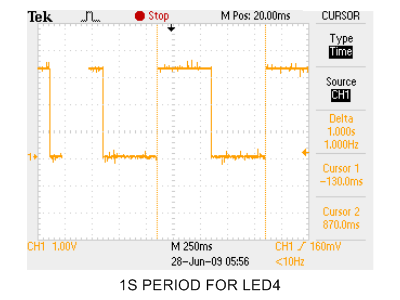
\includegraphics[width=0.4\textwidth]{period_led4.png}} \\                
  \subfloat[LED5 Period]{\label{fig:Per5}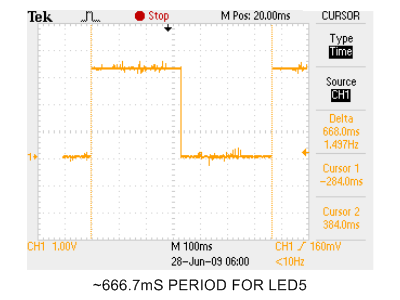
\includegraphics[width=0.4\textwidth]{period_led5.png}}
  \subfloat[LED6 Period]{\label{fig:Per6}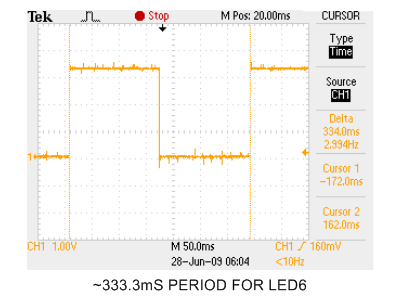
\includegraphics[width=0.4\textwidth]{period_led6.png}}
  \caption{Period of LED blink rate captured by osciliscope.}
  \label{fig:oscil}
\end{figure}

% INSERT SOURCE CODE
\lstset{language=Verilog, tabsize=3, backgroundcolor=\color{mygrey}, basicstyle=\small, commentstyle=\color{BrickRed}}
\lstinputlisting{MODULE.v}

% TEXT TABLE
\begin{table}
\begin{center}
\begin{tabular}{|l|c|c|l|}
	x & x & x & x \\ \hline
	x & x & x & x \\
	x & x & x & x \\ \hline
\end{tabular}
\caption{Caption}
\label{label}
\end{center}
\end{table}

% MATHMATICAL ENVIRONMENT
$ 8 = 2 \times 4 $

% CENTERED FORMULA
\[  \]

% NUMBERED EQUATION
\begin{equation}
	
\end{equation}

% ARRAY OF EQUATIONS (The splat supresses the numbering)
\begin{align*}
	
\end{align*}

% NUMBERED ARRAY OF EQUATIONS
\begin{align}
	
\end{align}

% ACCENTS
\dot{x} % dot
\ddot{x} % double dot
\bar{x} % bar
\tilde{x} % tilde
\vec{x} % vector
\hat{x} % hat
\acute{x} % acute
\grave{x} % grave
\breve{x} % breve
\check{x} % dot (cowboy hat)

% FONTS
\mathrm{text} % roman
\mathsf{text} % sans serif
\mathtt{text} % Typewriter
\mathbb{text} % Blackboard bold
\mathcal{text} % Caligraphy
\mathfrak{text} % Fraktur

\textbf{text} % bold
\textit{text} % italic
\textsl{text} % slanted
\textsc{text} % small caps
\texttt{text} % typewriter
\underline{text} % underline
\emph{text} % emphasized

\begin{tiny}text\end{tiny} % Tiny
\begin{scriptsize}text\end{scriptsize} % Script Size
\begin{footnotesize}text\end{footnotesize} % Footnote Size
\begin{small}text\end{small} % Small
\begin{normalsize}text\end{normalsize} % Normal Size
\begin{large}text\end{large} % Large
\begin{Large}text\end{Large} % Larger
\begin{LARGE}text\end{LARGE} % Very Large
\begin{huge}text\end{huge}   % Huge
\begin{Huge}text\end{Huge}   % Very Huge


% GENERATE TABLE OF CONTENTS AND/OR TABLE OF FIGURES
% These seem to have some issues with the "revtex4" document class.  To use, change
% the very first line of this document to "article" like this:
% \documentclass[aps,letterpaper,10pt]{article}
\tableofcontents
\listoffigures
\listoftables

% INCLUDE A HYPERLINK OR URL
\url{http://www.derekhildreth.com}
\href{http://www.derekhildreth.com}{Derek Hildreth's Website}

% FOR MORE, REFER TO THE "LINUX CHEAT SHEET.PDF" FILE INCLUDED!
